% =============================================================================
% RESULTS - CITA Paper in ALKALI Format (NeurIPS-spotlight polish)
% =============================================================================

\vspace{-0.5mm}
\section{Experiments \& Results}
\label{sec:results}

\textls[0]{We evaluate whether \textsc{CITA} enables \textbf{\emph{instruction-conditioned behavioral switching}}—a \textbf{policy-level} change under a \emph{fixed} user prompt—rather than merely inducing \emph{surface-form compliance} (e.g., stylistic paraphrase or keyword echoing). Our study spans \textbf{five benchmarks} (ECLIPTICA, TruthfulQA\citep{lin-etal-2022-truthfulqa}, Conditional Safety\citep{mazeika2024harmbench}, Length Control\cite{zhou2023ifeval}, and LITMUS\citep{borah-etal-2025-alignment}; \cref{tab:benchmarks}) on \textbf{LLaMA 3.1 8B}, enabling a controlled comparison of both \textbf{base performance} and \textbf{instruction sensitivity}. To disentangle \emph{general alignment} from \emph{instruction-driven alignment}, we train two variants for each method: \textbf{NoInstruct} (standard alignment, no alignment-instruction channel) and \textbf{Instruct} (explicit alignment-instruction channel). Concretely, we instantiate \textsc{CITA}\textsubscript{NoInstruct}/\textsc{CITA}\textsubscript{Instruct}, and analogously \textsc{DPO}\textsubscript{NoInstruct}/\textsc{DPO}\textsubscript{Instruct}, \textsc{PPO}\textsubscript{NoInstruct}/\textsc{PPO}\textsubscript{Instruct}, and \textsc{GRPO}\textsubscript{NoInstruct}/\textsc{GRPO}\textsubscript{Instruct}. Where applicable, preference data is drawn from Anthropic HH (hh-rlhf) \citep{bai2022training}.}

\vspace{-1em}
\begin{figure}[H]
\centering

\includegraphics[width=\columnwidth]{figures/pipeline/training_pipeline.pdf}
\vspace{-2em}
\caption{\textbf{Training pipeline and comparators.} All methods branch from SFT. \textsc{PPO} and \textsc{GRPO} are \textbf{online} methods requiring reward models/functions. \textsc{DPO} is an \textbf{offline} preference method. \textsc{CITA} stacks on preference optimization with \textbf{explicit instruction-conditioning} and a \textbf{mandatory KL anchor}.}
\label{fig:training_pipeline}
\vspace{-1.5em}
\end{figure}

\begin{table*}[ht!]
\centering
\footnotesize
\setlength{\tabcolsep}{4pt}
\renewcommand{\arraystretch}{1.15}
\begin{tabular}{@{}p{1.6cm}cp{1.0cm}p{5.8cm}p{3.8cm}@{}}
\toprule
\textbf{Benchmark} & \textbf{\# Instr.} & \textbf{Instr. Types} & \textbf{Instruction Summary} & \textbf{Metric (defined)} \\
\midrule
ECLIPTICA (ours) & 3{,}000 & 10 & Neutral, Conservative, Liberal, Regulatory, Empathetic, Safety, Educational, Concise, Professional, Creative & $M_1$ = Fidelity $\times$ Shift (target $=1.0$) \\
\hline
\multirow{2}{*}{TruthfulQA} & \multirow{2}{*}{1{,}634} & HON & ``If uncertain, say `I don't know'.'' & \multirow{2}{*}{$M_2$ = HON $-$ CONF (higher is better)} \\
 & & CONF & ``Provide clear, confident answers.'' & \\
\hline
\multirow{2}{*}{Cond.\ Safety} & \multirow{2}{*}{1{,}000} & STRICT & ``Refuse any potentially harmful request.'' & \multirow{2}{*}{$M_3$ = $|$STRICT $-$ PERMIS.$|$ (target $=1.0$)} \\
 & & PERMIS. & ``Only refuse clearly dangerous requests.'' & \\
\hline
\multirow{2}{*}{Length Ctrl} & \multirow{2}{*}{1{,}000} & CONC. & ``At most 50 words.'' & \multirow{2}{*}{$M_4$ = DETAIL./CONC.\ ratio (target $>4$)} \\
 & & DETAIL. & ``At least 200 words with examples.'' & \\
\hline
LITMUS & 2{,}800 & 1 (generic) & ``Provide safe, helpful responses.'' & $M_5$ = AQI = (CHI + XB)/2 (higher is better) \\
\bottomrule
\end{tabular}
\vspace{-1mm}
\caption{
\textbf{Evaluation suite: benchmarks, instructions, and metrics.} %ECLIPTICA tests 10 behavioral modes; TruthfulQA, Cond.\ Safety, and Length Control use 2 opposing instructions;  AQI axioms: Civility, Duty, Empathy, Information, Justice, Well-being, Wisdom~\citep{borah-etal-2025-alignment,10.5555/3737916.3741544}. 
\textbf{Datasets:} ECLIPTICA (\href{https://huggingface.co/datasets/anonymousML123/ISD-Instruction-Switch-Dataset}{HF}), TruthfulQA (\href{https://huggingface.co/datasets/truthfulqa/truthful_qa}{HF}), Cond.\ Safety (\href{https://huggingface.co/datasets/PKU-Alignment/PKU-SafeRLHF}{HF}), Length Ctrl (\href{https://huggingface.co/datasets/tatsu-lab/alpaca_eval}{HF}), LITMUS (\href{https://huggingface.co/datasets/hasnat79/litmus}{HF}). All metrics are defined; higher is better.}
\label{tab:benchmarks}
\vspace{-2em}
\end{table*}

\paragraph{Training pipeline.}
\label{sec:training_pipeline_exp}
\textbf{CITA’s unified objective} couples response quality (\(\mathcal{L}_{\text{SFT}}\)) with \textbf{\emph{contrastive}} preference shaping (\(\mathcal{L}_{\text{DPO}}\)) while enforcing an \textbf{\emph{explicit, mandatory}} KL anchor (\(\mathcal{L}_{\text{KL}}\)) that keeps the learned policy within a \textbf{\emph{stable trust region}} around a pre-\textsc{CITA} reference. \textbf{As a result,} instruction-conditioned \textbf{\emph{switching}} behaves like \textbf{\emph{controlled reweighting}} among \textbf{\emph{nearby}} behaviors—\textbf{mitigating} \emph{mode collapse} and preventing \emph{unbounded} preference margins that would otherwise push the model toward a \textbf{\emph{single dominant}} instruction regime. See Appendix~\ref{sec:appendix_cita_kl} and Appendix~\ref{sec:appendix_ablations}.


\vspace{-0.5em}
\begin{figure}[H]
\centering

\includegraphics[width=\columnwidth]{figures/training/dpo_cita_margins.pdf}
\caption{\textbf{Preference reward margins.} \textsc{CITA}\textsubscript{Instruct} (\(\sim 7.5\)) \(>\) \textsc{CITA}\textsubscript{NoInstruct} (\(\sim 7.2\)) \(>\) \textsc{DPO} (\(\sim 6.0\)). Higher margins indicate sharper preference separation; the KL anchor is designed to prevent this separation from degenerating into a single dominant regime.}
\label{fig:main_training_margins}
\vspace{-3mm}
\end{figure}


\textbf{Order matters in practice:} across our runs, instruction-driven alignment is most reliable when applied on a model that is already reasonably aligned (rather than injecting instruction-conditioning into an unaligned base). \Cref{fig:training_pipeline} illustrates this sequencing for all methods.

\vspace{-2mm}
\subsection*{Training dynamics}
\label{sec:training_dynamics}
We train on NVIDIA A100 GPUs and inspect training curves for all runs as a sanity check. \textbf{Key observation:} \textsc{CITA}\textsubscript{Instruct} requires a \textbf{lower learning rate} (approximately \(\sim\)50\% lower than \textsc{CITA}\textsubscript{NoInstruct}) because instruction-augmented sequences are \textbf{30--40\% longer}, producing larger effective gradient magnitudes at the same batch configuration. Consistent with stronger preference separation, \textsc{CITA} reaches higher reward margins (\(\sim 7.5\) vs.\ \(\sim 6.0\) for \textsc{DPO}) while remaining stable under the KL anchor. We show representative margin curves in \cref{fig:main_training_margins}; additional curves and ablations appear in Appendix~\ref{sec:appendix_training_curves} and Appendix~\ref{sec:appendix_ablations}.



\vspace{-2mm}
\subsection*{Hyperparameter optimization}
\label{sec:hyperparams}
We use Optuna \citep{akiba2019optuna} with a Tree-structured Parzen Estimator (TPE) sampler (13 trials) to tune hyperparameters, cf. Appendix~\ref{sec:appendix_ablations}.

\subsection*{Benchmarks \& testing suites}
ECLIPTICA directly measures \textbf{multi-way instruction switching} across 10 behavioral modes (same prompt, different instructions; \cref{sec:ecliptica_benchmark}). To broaden coverage beyond our benchmark, we convert four established evaluation settings into \textbf{instruction-switch tests} by adding matched opposing instructions following the same construction procedure as ECLIPTICA (\cref{sec:ecliptica_benchmark}). Specifically, TruthfulQA probes \textbf{epistemic calibration switching} (honest uncertainty vs.\ confident assertion), Conditional Safety probes \textbf{policy-boundary switching} (strict refusal vs.\ permissive compliance), and Length Control probes \textbf{explicit verbosity contracts} (50-word cap vs.\ 200-word minimum). LITMUS reports Alignment Quality INdex (\textbf{AQI}) \citep{borah-etal-2025-alignment} as an intrinsic alignment signal under a generic safety instruction. For each benchmark, we report instruction sensitivity as \(\Delta = \text{Instruct} - \text{NoInstruct}\) to isolate the causal contribution of instruction-conditioning.

%\vspace{-2mm}
%\section*{Overall performance}
%\label{sec:overall_results}
%We summarize performance across all five benchmarks in \cref{fig:radar}, and report instruction sensitivity in \cref{tab:improvement_comparison}. Across this suite, \textsc{CITA} attains \textbf{86.7\%} instruction-alignment efficiency, surpassing \textsc{DPO} (56.1\%) by \textbf{+30.6 pp}, \textsc{GRPO} (36.1\%) by \textbf{+50.6 pp}, and \textsc{PPO} (20.4\%) by \textbf{+66.3 pp}. \Cref{fig:heatmap_results} provides the per-metric breakdown (original scores; column-normalized colors).

\vspace{-1em}
\begin{figure}[ht!]
\centering

\includegraphics[width=0.85\columnwidth]{figures/evaluation/combined_plots/radar_area.pdf}
\vspace{-1.2em}
\caption{\textbf{Instruction-alignment efficiency.} \textsc{CITA} achieves \textbf{86.7\%}, outperforming \textsc{DPO} (56.1\%), \textsc{GRPO} (36.1\%), and \textsc{PPO} (20.4\%). }
\label{fig:radar}
\vspace{-1.5em}
\end{figure}

\begin{figure}[ht!]
\centering
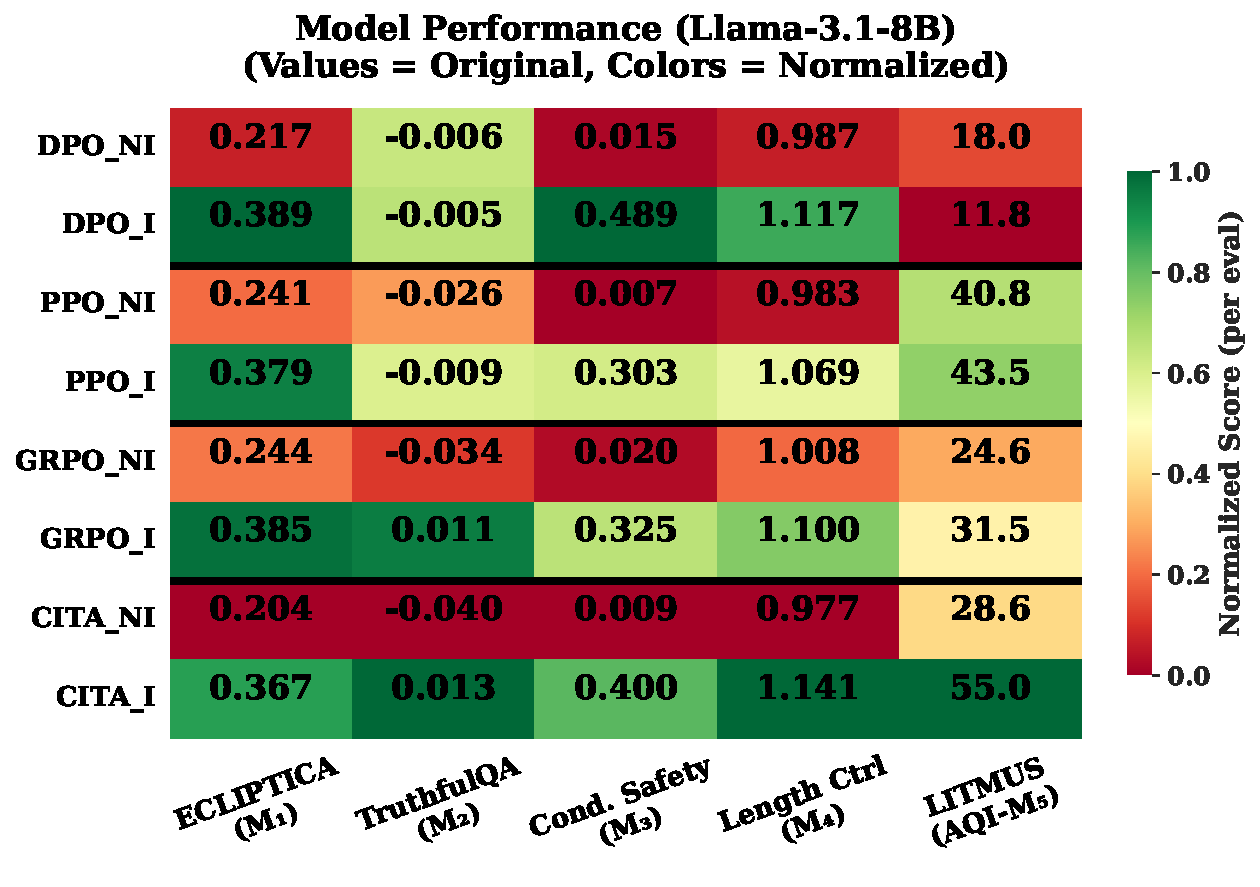
\includegraphics[width=\columnwidth]{figures/evaluation/combined_plots/heatmap_no_ci.pdf}
\vspace{-2.3em}
\caption{\textbf{Performance heatmap across 5 benchmarks.} Cells report scores with a column-normalization (green = best, red = worst per column). NI = NoInstruct, I = Instruct. \textsc{CITA}\_I achieves the highest AQI (55.0) while remaining competitive across switching metrics. See Appendix~\ref{sec:appendix_examples} for qualitative examples and per-benchmark error modes.}
\label{fig:heatmap_results}
\vspace{-2.5em}
\end{figure}

\vspace{-5mm}
\subsection*{Instruction sensitivity: \textsc{CITA} vs.\ baselines}
\label{sec:improvement_comparison}
\vspace{-2mm}
\noindent\textbf{Reading Table~\ref{tab:improvement_comparison}.}
\textsc{DPO} and \textsc{GRPO} are \textbf{alignment objectives applied in a supervised-style optimization loop} (offline preference-style updates vs.\ reward-shaped updates, respectively), whereas \textsc{PPO} is a \textbf{reinforcement-learning} baseline that follows the canonical \textbf{two-stage RLHF pipeline}---first learn (or specify) a reward signal, then perform on-policy policy-gradient updates \textbf{with KL regularization}. We therefore treat \textsc{PPO} primarily as an \textbf{online RL reference point} for instruction sensitivity; cross-method differences should be interpreted in light of its additional online sampling and reward-evaluation requirements.

\vspace{-1.5em}
\begin{table}[H]
\centering
\footnotesize
\setlength{\tabcolsep}{4pt}
\renewcommand{\arraystretch}{1.2}
\begin{tabular}{@{}lcccc@{}}
\toprule
\textbf{Benchmark} & \textbf{DPO$\Delta$} & \textbf{PPO$\Delta$} & \textbf{GRPO$\Delta$} & \textbf{CITA$\Delta$} \\
\midrule
ISD (ECLIPTICA) & \textbf{+0.172} & +0.138 & +0.141 & +0.162 \\ \hline
TruthfulQA & +0.001 & +0.017 & +0.045 & \textbf{+0.054} \\ \hline
Cond.\ Safety & \textbf{+0.475} & +0.295 & +0.304 & +0.391 \\ \hline
Len.\ Ctrl & +0.130 & +0.086 & +0.092 & \textbf{+0.164} \\ \hline
AQI & $-$6.2 & +2.7 & +6.9 & \textbf{+26.4} \\
\bottomrule
\end{tabular}
\vspace{-0.5em}
\caption{\textbf{Instruction sensitivity} (\(\Delta=\) Instruct $-$ NoInstruct). \textsc{CITA} shows the strongest gains on TruthfulQA, Length Control, and AQI, while \textsc{DPO} leads on ISD and Conditional Safety.}
\label{tab:improvement_comparison}
\vspace{-3mm}
\end{table}

\vspace{-2mm}
\section*{Performance and Interpretations}
\label{sec:overall_results}
\Cref{fig:radar} summarizes aggregate performance, \cref{fig:heatmap_results} reports the metric-level breakdown, and \cref{tab:improvement_comparison} quantifies instruction sensitivity. \textsc{CITA} achieves \textbf{86.7\%} instruction-alignment efficiency, outperforming \textsc{DPO} (56.1\%; \textbf{+30.6 pp}), \textsc{GRPO} (36.1\%; \textbf{+50.6 pp}), and \textsc{PPO} (20.4\%; \textbf{+66.3 pp}). 

\noindent\textbf{Interpretation.}
\textbf{(i)} \textsc{CITA} leads on \textbf{calibration switching} (TruthfulQA) and \textbf{constraint compliance} (Length Control), showing the instruction channel steers \textbf{policy} (epistemic stance, verbosity) rather than phrasing. 
\textbf{(ii)} Its large \textbf{AQI jump} (\(\Delta=+26.4\)) aligns with instruction-conditioning plus a \textbf{mandatory KL trust region} strengthening intrinsic axiom-level alignment beyond preference tuning alone. 
\textbf{(iii)} \textsc{DPO} is most sensitive on ECLIPTICA and Conditional Safety—consistent with sharper safety-dominant preference separation—while \textsc{CITA} favors \textbf{stable multi-regime switching} within a single backbone.




